\section{\textit{Filters}}

En el campo de la síntesis sonora, tan importante es la generación de una señal a partir de la suma de otras, como la capacidad de filtrar componentes espectrales de una señal dada. Ambos caminos, basados en el hecho de que cualquier señal periódica imaginable puede ser descompuesta en una suma de señales sinusoidales, constituyen la \textit{síntesis aditiva} y la \textit{síntesis sustractiva} respectivamente. Son los filtros los módulos imprescindibles en la síntesis sustractiva, ya que permiten elegir un grupo de frecuencias de entre todas las que ofrece la señal de su entrada, generando cambios tímbricos y dinámicos en la señal de salida.

\subsection{Tipos de filtros}

No es este el lugar para profundizar mundo del filtrado de señales, por su complejidad y amplitud. Simplemente se darán unas pinceladas básicas para poder describir el comportamiento del módulo \textit{filter} de Synthi 100.

De igual modo que una señal luminosa puede ser descompuesta en diferentes longitudes de onda, formando líneas o bandas espectrales, el sonido también se puede representar en el dominio de la frecuencia, de manera que es susceptible de ser descrito como la suma de un número ilimitado de componentes sinusoidales, con su propia amplitud y fase. Los diferentes \textit{timbres} o \textit{colores} de un sonido están fuertemente determinados por esta composición frecuencial. Filtrar un sonido o señal no será otra cosa que dejar pasar ciertas frecuencias de una señal y cancelar otras, consiguiendo un producto sonoro diferente de la señal original a nivel tímbrico.

A grandes rasgos, los tres tipos de filtros más importantes (Fig. \ref{fig:filtersgraph}) son el \textit{de paso bajo} (LPF), el \textit{de paso alto} (HPF) y el \textit{de paso banda} (BPF). Los dos primeros tiene la característica común de dejar pasar solo las componentes frecuenciales de un lado del espectro, bien del lado de los graves (bajos), bien del lado de los agudos (altos), teniendo como principal parámetro la \textit{frecuencia de corte}, a partir de la cual se atenúan o cancelan el resto de frecuencias. El filtro \textit{de paso de banda} tiene como variables una frecuencia central y una anchura de la banda que deja pasar. Otros parámetros importantes determinan el tipo de curva y de pendiente que tiene el filtro en su frecuencia de corte, lo que queda determinado, principalmente, por su \textit{orden}. 

\begin{figure}
	\centering
	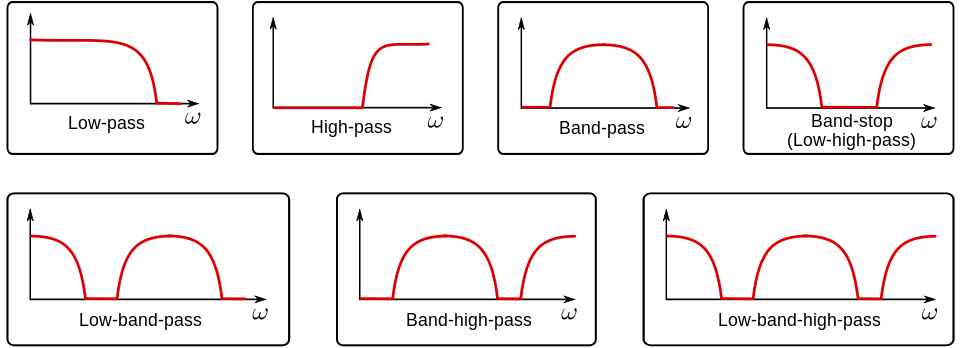
\includegraphics[width=0.7\textwidth]{images/filtersgraph}
	\caption[Tipos de filtro]{Diferentes tipos de filtro. De izquierda a derecha en la fila superior: \textit{pasa bajo}, \textit{pasa alto}, \textit{pasa banda} y \textit{rechaza banda}. En la fila inferior, diversos filtros producto de combinaciones de otros más simples (imagen original de SpinningSpark, CC BY-SA 3.0, modificada por el autor).}
	\label{fig:filtersgraph}
\end{figure}

A partir de estos filtros teóricos, la tecnología en torno al filtrado de señales ha combinado de múltiples maneras todos sus parámetros en función de sus objetivos. Se pueden encontrar filtros en los que puede variar uno o varios de sus parámetros (frecuencia de corte, anchura de banda...), combinados en filtros \textit{multibanda}, filtros en serie que provocan un cambio en el \textit{orden} del filtrado, filtros de \textit{rechazo de banda} (como una combinación de LPF y HPF), etc.

Por último, conviene indicar la exitencia de filtros en los que la frecuencia de corte puede tener una amplitud adicional, formando un pico más o menos pronunciado. Esta amplitud es conocida como \textit{resonancia}. En los sintetizadores analógicos, si esta resonancia es lo suficientemente elevada, se puede producir un sonido sinusoidal en la frecuencia de corte incluso en la ausencia de señal de entrada. Esta característica es utilizada por EMS en varios de sus dispositivos, entre ellos el Synthi 100.


\subsection{Los filtros resonantes de Synthi 100}

El Synthi 100 cuenta en su primer panel con 8 módulos denominados \textit{filter}, cada uno de los cuales permite variar tres parámetros: \textit{Frequency}, \textit{Response} y \textit{Level} (Fig. \ref{fig:filters}). Estos 8 módulos están divididos en dos grupos de 4: \textit{Low pass/Resonator/Osc}, con los filtros del 1 al 4, y \textit{High pass/Resonator/Osc}, con los numerados del 5 al 8.

\begin{figure}
	\centering
	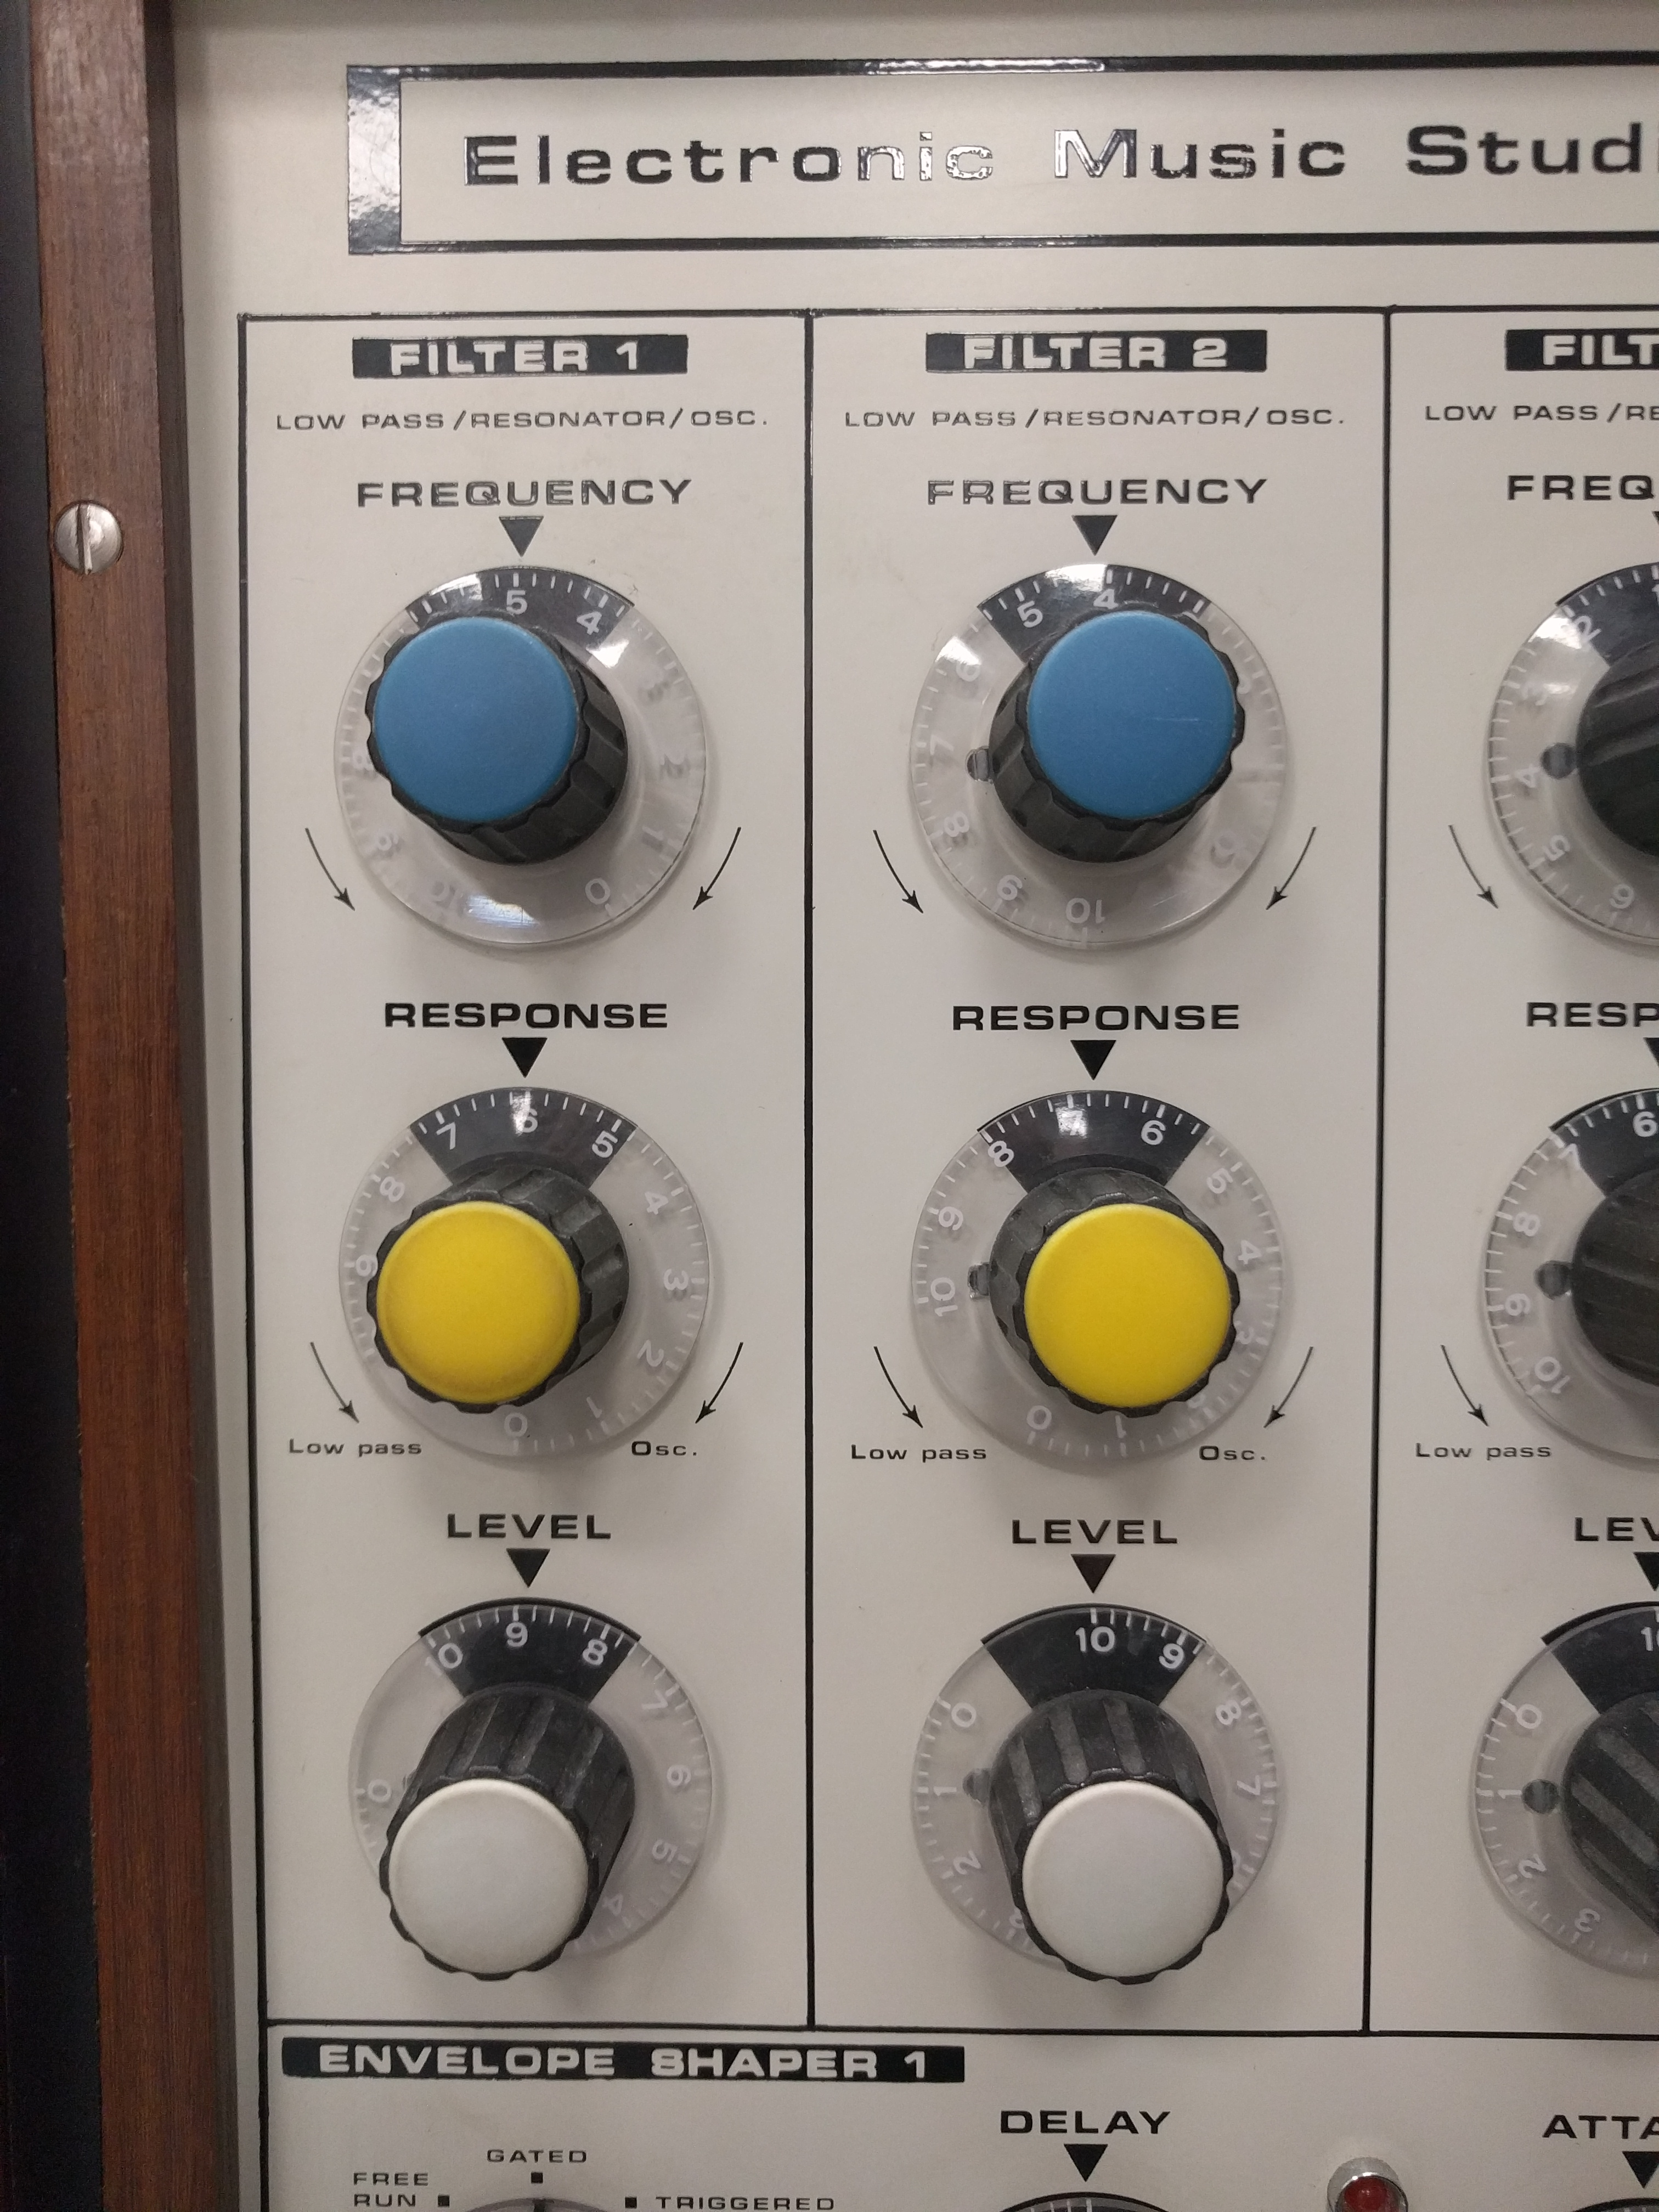
\includegraphics[width=0.4\textwidth]{images/filters}
	\caption{Dos de los 8 filtros del Synthi 100 del GME.}
	\label{fig:filters}
\end{figure}

Para comprender mejor el comportamiento de este módulo, a continuación se describe el comportamiento del dial \textit{Frequency} en función de los diversos valores de \textit{Response}:

\begin{description}
	\item[\textit{Low/Hith pass} ($\textit{Response} \gtrapprox 0$)] El filtro se comporta como \textit{Low pass} (filtros 1 al 4) o \textit{High pass} (filtros 5 al 8). \textit{Frequency} varía la frecuencia de corte del filtro.
	\item[\textit{Resonator} ($\textit{Response} \approx 5$)] En torno al valor de 5, el filtro se comporta como \textit{Low} o \textit{High pass} con amplificación de la frecuencia de corte.
	\item[\textit{Osc} ($\textit{Response} \lessapprox 10$)] A medida que el valor de \textit{Response} se acerca a 10, el resultado se acerca a un sonido sinusoidal cuya frecuencia es \textit{frequency}. El filtro se comporta prácticamente como un oscilador incluso cuando no existe una señal de entrada. 
\end{description}

\subsection{Implementación en Supercollider}

Existen diversos UGens que pueden emular perfectamente el comportamiento de un filtro \textit{resonante}, es decir, del tipo \textit{de paso bajo} o \textit{de paso alto} con la adición de la amplificación de la frecuencia de corte. Se ha optado por usar los filtros \texttt{BLowPass} y \texttt{BHiPass} respectivamente. Estos forman parte del conjunto de filtros \textit{BEQSuite}, incluidos en las distribuciones estándar de SuperCollider. 

Existe, sin embargo, cierto comportamiento de los filtros resonantes analógicos que no es posible emular con estos filtros digitales: la posibilidad de convertirse en un oscilador cuando el valor de su resonancia se acerca al máximo sin contar con la existencia de una señal de input. Habitualmente, la salida de un filtro digital en estas circunstancias será nula. Para emular esta característica analógica, se ha añadido un ruido blanco constante de una amplitud casi insignificante (en torno a $-60 dB$). Este nivel de ruido es suficiente como para ser amplificado como para convertirse en señal audible en en la frecuencia de corte cuando el valor de \textit{response} se acerca a 10.






